\documentclass[11pt]{article}

\usepackage[a4paper,margin=2.6cm]{geometry}
\usepackage[T1]{fontenc}
\usepackage[utf8]{inputenc}
\usepackage{lmodern}
\usepackage{microtype}
\usepackage{amsmath,amssymb}
\usepackage{booktabs}
\usepackage{graphicx}
\usepackage{xcolor}
\usepackage[font=small,labelfont=bf]{caption}
\usepackage{enumitem}
\definecolor{linkblue}{HTML}{1c5cab}
\usepackage[colorlinks=true,linkcolor=linkblue,citecolor=linkblue,urlcolor=linkblue]{hyperref}

\newcommand{\sillage}{\textsc{Sillage}}
\newcommand{\dnll}{\Delta\mathrm{NLL}}
\newcommand{\ci}[2]{{\footnotesize[#1,\,#2]}}

\title{\bfseries The Memory Pays for Itself:\\
Cross-Model Recall and Exact Speculative Acceleration\\
from One Fixed-Size Hebbian State}
\author{Abderrahmane Sghairi\\
\small Independent Researcher, Issoire, France\\
\small \texttt{sghairipro63@gmail.com}}
\date{August 2026\\[2pt]
\small DOI: \href{https://doi.org/10.5281/zenodo.22109220}{10.5281/zenodo.22109220}
\qquad Code: \href{https://github.com/riscoss63/sillage}{github.com/riscoss63/sillage}}

\begin{document}
\maketitle

\begin{abstract}
Four companion papers gave frozen language models a gradient-free, fixed-size memory --- a Hebbian matrix with vector-symbolic $n$-gram keys, square-root amplitude values, and writes gated by the model's own surprise --- that improves prediction on text the model has read. This paper shows that the \emph{same state, unchanged}, pays for itself twice more. \textbf{(1) It transfers across a model family.} A 25\,MB state written by Qwen3-0.6B while reading two manuscripts, mixed into the logits of Qwen3-1.7B (which read nothing), lets the bigger model recall those documents: two minutes of \emph{read-only} calibration --- the papers' published tuning grids, fitted teacher-forced on a 20\% dev window --- take the 1.7B's dev NLL from $2.147$ alone to $0.360$ (perplexity $8.6 \to 1.4$), and verbatim regeneration of the source rises $+27\%$ outside the calibration window. The same automatic calibration, run for Qwen3-4B, selects the same settings, replicating the recall at a third model size. \textbf{(2) It accelerates generation, exactly.} Used as a drafter for speculative decoding --- the cold store proposing exact continuations, the Hebbian matrix proposing above its own abstention threshold, the augmented model verifying a block per forward --- the state converts its confidence into wall-clock speed with output \emph{identical} to normal greedy decoding, by construction and verified. On a T4 GPU, where we measure that verifying 16 tokens costs the same as verifying one (ratio $0.94$), acceptance rates of 70--87\% yield end-to-end speedups of $\times$1.63 (0.6B), $\times$\textbf{1.98} (1.7B), and $\times$1.86 with 87\% acceptance (4B) on document-grounded generation, at $0.52$--$0.65$ target forwards per emitted token --- while a vanilla-target control shows $\times$1.14 at 30\% acceptance (a drafter cannot accelerate beliefs its target does not hold), and unseen-text controls sit at $\times$0.97--1.09 (speculation never costs). Four negative results are documented: loosening the draft gate destroys the gain (precision beats coverage); accelerating an unaugmented target fails; fp16 argmax ties break output identity on GPT-2 (2 of 15 prompts; zero of 60 on Qwen3); and a prompt-lookup baseline's apparent wins are partly an artifact of greedy degeneration. A fifth, structural finding: on a 2-core host the vocabulary-sized readout costs three times the GPU forward itself, so the memory must live on the accelerator --- our torch port of the readout triples even non-speculative throughput. Code and all result files are released; the states rebuild by reading (the papers state with one command --- the Manuscripts stream, as throughout this series, is not redistributed).
\end{abstract}

\section{Introduction}

The companion papers of this series \cite{sillage,router,hier,fw} equip a frozen language model with a fixed-size, gradient-free memory: a Hebbian matrix addressed by sliding vector-symbolic $n$-gram bindings, storing square-root amplitudes, written once per token under a gate equal to the model's own surprise $-\ln p_{\mathrm{LM}}$, with an exact cold store consolidated by surprise mass \cite{hier} and a rank-16 delta-rule readout adapter \cite{fw}. Those papers measured one currency: prediction quality on the stream being read.

This paper measures two different currencies for the \emph{same} state, without changing a single write rule.

First, \textbf{whose model is it, anyway?} The memory lives in a model's \emph{token space}, not in its weights: keys and values are functions of token identities alone. Any model sharing the tokenizer can therefore read it. We ask what a state written by a small, cheap reader (Qwen3-0.6B) is worth to its larger siblings (Qwen3-1.7B and 4B, same 151{,}936-token vocabulary) --- and what it takes to connect them. The answer is a read-only calibration: the tuning protocol of the companion papers (grids over the mixing weight, temperature and abstention threshold), run teacher-forced on a dev window with \emph{no writes}, in about two minutes.

Second, \textbf{can the memory pay for its keep in wall-clock time?} Speculative decoding \cite{leviathan,chen} converts a cheap guesser into speed: a drafter proposes $k$ tokens, the target verifies them in one forward pass, and greedy verification reproduces the target's output token for token. Our drafter costs no model call at all --- the cold store proposes exact continuations of the current 4-gram, the Hebbian matrix proposes its argmax above the abstention machinery the readout already carries --- and, unlike every deployed retrieval drafter we know of \cite{pld,rest,suffix,nest,omnidraft}, it is \emph{persistent across sessions, fixed in size, and written by reading}, not by observing the serving stream.

\paragraph{Contributions.}
\begin{enumerate}[leftmargin=1.5em,itemsep=2pt]
\item \textbf{Cross-model state transfer with read-only calibration} (\S\ref{sec:transfer}): the 0.6B's state gives the 1.7B a dev NLL of $0.360$ against $2.147$ alone (PPL $8.6 \to 1.4$), with verbatim source regeneration up $+27\%$ \emph{outside} the calibration window; the automatic calibration selects the same settings for the 4B, and the vanilla control shows the effect is entirely the memory's ($0.4$ words of verbatim recall without it).
\item \textbf{An exact speculative drafter from the state alone} (\S\ref{sec:drafter}): draft acceptance of 70--87\% across four target models on document-grounded generation, with output identity to plain greedy decoding verified on every run (60/60 Qwen3 outputs; the fp16 caveat of \S\ref{sec:negative} on GPT-2).
\item \textbf{The conversion factor, measured} (\S\ref{sec:micro}): on a T4, one forward over 16 draft tokens costs $0.94\times$ a single-token forward --- verification is free --- and end-to-end speedups follow: $\times$1.63 / $\times$1.98 / $\times$1.86 at the three Qwen3 sizes, $\times$1.36 on GPT-2, within 2--4\% of the bound implied by the round statistics at the Qwen3 sizes (\S\ref{sec:speed}).
\item \textbf{A systems result} (\S\ref{sec:ondevice}): with a 151{,}936-token vocabulary, the numpy readout (one matrix--vector scoring plus mixing per position) costs $\sim$130\,ms/token on a 2-core host --- three times the GPU forward itself. Porting keys, values, scoring, mixing and batched verification to the accelerator triples even non-speculative throughput and is what makes the speedups above realizable.
\item \textbf{Four negative results} (\S\ref{sec:negative}), reported as boundaries: a looser draft gate lowers both acceptance and speed; a vanilla (un-augmented) big target cannot be usefully accelerated by the small reader's memory; fp16 argmax ties can break exact output identity on older architectures; and prompt-lookup baselines are flattered by greedy degeneration, a hazard for every speculative-decoding evaluation that reports on open-ended generation.
\end{enumerate}

\section{Related work}

\textbf{Speculative decoding.} Draft-and-verify with rejection guarantees is due to \cite{leviathan,chen}. Model-free drafters retrieve rather than compute: prompt-lookup copies the continuation of the current $n$-gram from the live context \cite{pld}; REST retrieves from a fixed external datastore \cite{rest}; SuffixDecoding grows per-deployment suffix trees over the serving stream, unbounded, server-side \cite{suffix}; NEST drafts spans from a nonparametric index with attribution \cite{nest}; OmniDraft adapts a small drafter online by gradient distillation \cite{omnidraft}. Our drafter occupies the unclaimed corner: \emph{no gradients, fixed bytes ($\le$25\,MB), persistent across sessions, written by reading documents rather than by watching outputs} --- and it is the same object that improves the target's predictions, so drafting confidence and prediction confidence share one calibration.

\textbf{Memory for frozen models.} kNN-LM \cite{khandelwal2020} and the companion papers \cite{sillage,router,hier,fw} modify a frozen model's output distribution; test-time-memorization architectures \cite{titans,ttt} learn theirs with gradients; Cartridges \cite{cartridges} distill a corpus into a trained KV artifact offline. Cross-model reuse of a \emph{token-space} state, to our knowledge, has not been reported: hidden-state datastores (kNN-LM) and trained artifacts (Cartridges) are bound to the network that produced them, whereas the state used here binds only to the tokenizer.

\textbf{Models.} Frozen GPT-2 124M \cite{gpt2} and the Qwen3 family (0.6B, 1.7B, 4B; shared vocabulary) \cite{qwen3}.

\section{Method}

\subsection{The state, unchanged}

Everything is inherited from the companion papers and none of it is modified here: the $4096 \times 256$ Hebbian matrix $M$ with sliding 4-gram hypervector keys and amplitude (square-root-of-mass) values \cite{sillage}; the bounded exact cold store mapping 4-grams to successor counts, consolidated by surprise mass \cite{hier}; the rank-16 readout adapter \cite{fw} (used only when the reading model itself is the target; it is a function of that model's hidden geometry and cannot transfer); and the score-level mixing interface with per-tier confidence abstention \cite{router}:
\begin{equation}
p \;=\; \mathbf{1}[s_{\max} \ge \theta]\,\lambda\, p_{\mathrm{mem}} + \bigl(1 - \mathbf{1}[\cdot]\,\lambda\bigr)\, p_{\mathrm{base}},
\qquad p_{\mathrm{mem}} = \mathrm{softmax}(\beta s),
\label{eq:mix}
\end{equation}
followed by the cold store's empirical successor distribution at fixed weight where its gram is present. Generation never writes.

\subsection{Cross-model transfer and read-only calibration}\label{sec:transfermethod}

Keys and values are deterministic functions of token identities (hypervectors regenerated from seeds), so any causal model with the same tokenizer can read the state through Eq.~\eqref{eq:mix}; the only model-bound quantities are the readout settings $(\beta, \lambda, \theta)$, which the companion papers tune per model. We connect a new target with the papers' own protocol, run \emph{read-only}: teacher-force the target over the first 20\% of the lifetime stream (here 3{,}380 tokens, one position in three retained, 1{,}127 observations), record the base probability of the truth and the memory's scores, and search the published grids for the $(\beta, \lambda, \theta)$ minimizing dev NLL. Nothing is written; nothing is saved; the cost is a prefill --- about two minutes on the hardware of \S\ref{sec:protocol}.

\subsection{The drafter, and exact block verification}\label{sec:draftermethod}

At each round the drafter proposes up to $\gamma = 8$ tokens using the state alone, no model call: first the \textbf{cold store} --- if the current 4-gram is present with $\ge 2$ occurrences and its majority successor holds probability $\ge 0.35$, propose it (chains may continue to $\gamma$) --- else the \textbf{matrix} --- if the retrieval score clears the 75th-percentile confidence threshold the readout already maintains, propose its argmax, at most twice consecutively. The sliding key advances over the drafter's own proposals and is snapshot-rewound on rejection.

The target then scores the whole draft block in \emph{one} forward pass. For greedy decoding, position $i$ is accepted while the target's argmax --- computed from the full augmented distribution of Eq.~\eqref{eq:mix}, exactly as in plain decoding --- equals the drafted token; the first disagreement emits the target's own token instead, and a fully accepted block emits the free bonus token \cite{leviathan}. The KV cache is cropped to the accepted prefix. Consequently the output is \emph{identical} to plain greedy decoding of the same augmented target, whatever the drafter does; we assert this identity on every run. Speculation can change speed, never content.

\subsection{The conversion factor}\label{sec:micromethod}

Let $c(k)$ be the latency of one forward over $k$ tokens with a warm KV cache. Speculative decoding replaces, per round, several single-token forwards by one $c(k{+}1)$; its ceiling is governed by $c(k)/c(1)$. On CPU, $c(k) \approx k\,c(1)$ (compute-bound): the only saving is per-call overhead, and we measured $\times$1.41 at best there. On an accelerator, decoding is latency-bound and $c(16)/c(1) \approx 1$: every accepted token is nearly free. We measure $c(k)$ directly (\S\ref{sec:micro}) rather than assume it.

\section{Protocol}\label{sec:protocol}

\textbf{States.} (i) \texttt{memory\_state}: written by frozen Qwen3-0.6B reading two versions of an unpublished technical manuscript (16{,}900 tokens lifetime; 9{,}883 cold grams; the adapter trained alongside) --- novel to every model used here. (ii) \texttt{papers\_state}: written by frozen GPT-2 124M reading the four companion preprints (21{,}832 tokens; 18{,}230 grams). States are not shipped in the repository --- a state's cold store maps $n$-grams to successors, so releasing one would release the text it read; the papers state rebuilds with one command (\texttt{sillage papers --with-memory}), and the protocol runs unchanged on any two documents of the reader's own (the Manuscripts stream itself, as throughout this series, is not redistributed).

\textbf{Prompts.} \emph{Seen}: 10 windows of 24 consecutive words sampled at fixed seeded offsets from the read documents; each generation runs 28 tokens, greedy. \emph{Unseen} (control): 5 generic English sentences the states never read. We also record, per seen prompt, how many leading words of the plain generation reproduce the source document verbatim (``verbatim recall''), and we flag the 4 of 10 prompts whose position overlaps the calibration window, reporting recall inside and outside that window separately.

\textbf{Configurations.} \textbf{A}: 0.6B generating with its own state (adapter on). \textbf{B}: 1.7B \emph{vanilla} --- the memory only drafts; the target's distribution is untouched (the pure-acceleration control). \textbf{C}: 1.7B or 4B with the 0.6B's state mixed in (adapter off), readout either inherited from the 0.6B or calibrated per \S\ref{sec:transfermethod}. \textbf{GPT-2}: self-target on \texttt{papers\_state}. Baseline drafter: prompt-lookup \cite{pld} over the live context (the no-persistence ablation), verified by the identical machinery.

\textbf{Hardware and engines.} CPU: 16-thread laptop, fp32, numpy readout (the reference implementation, cross-checked). GPU: Kaggle T4, fp16, with the readout resident on the device (\S\ref{sec:ondevice}); the torch engine reproduces the numpy engine's outputs token-for-token in fp32, including speculative paths and cold-store rounds. All numbers in this paper are committed as JSON in \texttt{results/} (\texttt{drafter\_*.json}) and regenerate from released scripts with fixed seeds.

\section{Results}

\subsection{A small reader's memory serves its bigger siblings}\label{sec:transfer}

\begin{figure}[t]
\centering
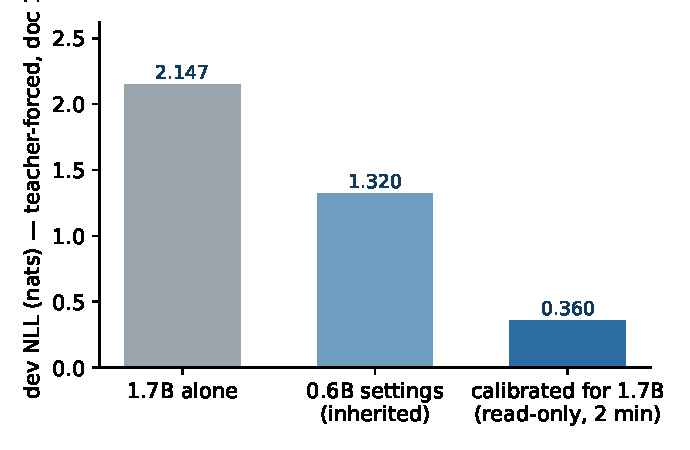
\includegraphics[width=0.55\linewidth]{figs/p5fig3_calibration.pdf}
\caption{Read-only calibration connects the 0.6B's state to the 1.7B: dev NLL (teacher-forced on the calibration window) of the 1.7B alone, with the state under the 0.6B's published settings, and with settings fitted for the 1.7B ($\beta\,160 \to 40$, $\lambda\,0.2 \to 0.85$, threshold $q_{75} \to q_{50}$). The fitted mix trusts the memory at the top of the grid --- the same response the tuner gave the 0.6B itself in \cite{sillage}.}
\label{fig:calib}
\end{figure}

Figure~\ref{fig:calib}: on the dev window, the 1.7B alone scores NLL $2.147$; the 0.6B's state under \emph{inherited} settings already brings it to $1.320$; two minutes of read-only calibration reach $\mathbf{0.360}$ --- perplexity $8.6 \to 1.4$ on the document the state knows. The behavioral counterpart is verbatim recall: the vanilla 1.7B regenerates $0.4$ leading words of the source on average (it read nothing --- the control that attributes everything that follows to the state); with the state under inherited settings, $3.7$ words; calibrated, $5.5$. Splitting by the calibration window: \emph{outside} it, recall goes $3.0 \to 3.8$ ($+27\%$ --- the calibration generalizes); inside it, $4.8 \to 8.0$. Run for the 4B, the same automatic calibration selects the \emph{same} settings $(\beta{=}40, \lambda{=}0.85, q_{50})$ and yields $5.6$ words of recall: the connection procedure is stable across the family. On unseen text every configuration behaves like its base model --- at $\lambda = 0.85$ the abstention machinery and the near-orthogonality of the keys keep the memory silent where it knows nothing (measured, not assumed: the 4B accepts $0$ of $16$ drafts there and its cold store never fires).

\subsection{Acceptance: the drafting signal across four targets}\label{sec:drafter}

\begin{table}[t]
\centering\small
\caption{Draft acceptance on seen streams (greedy, $\gamma = 8$, 10 prompts $\times$ 28 tokens), by source. Identity: speculative output vs plain decoding of the same target. CPU and GPU agree on every acceptance figure; outputs are engine-identical in fp32.}
\label{tab:acc}
\begin{tabular}{@{}llccc@{}}
\toprule
target & state / settings & acceptance & cold store & matrix\\
\midrule
Qwen3-0.6B (self, adapter on) & own & 76\% (110/144) & 79\% (90/114) & 67\% (20/30)\\
Qwen3-1.7B $+$ state & calibrated & 75\% (165/219) & 75\% (140/186) & 76\% (25/33)\\
Qwen3-1.7B $+$ state & inherited & 60\% (87/145) & 60\% (75/125) & 60\% (12/20)\\
Qwen3-4B $+$ state & auto-calibrated & \textbf{87\% (158/182)} & 88\% (140/160) & 82\% (18/22)\\
Qwen3-1.7B vanilla (control) & --- & 30\% (24/79) & 28\% (16/57) & 36\% (8/22)\\
GPT-2 (self, adapter on) & own & 70\% (78/111) & 71\% (10/14) & 70\% (68/97)\\
\bottomrule
\end{tabular}
\end{table}

Table~\ref{tab:acc}: where the target carries the memory, 70--87\% of drafted tokens are accepted, and calibration is what aligns drafter and target ($60\% \to 75\%$ on the 1.7B). The cold store is the precision source on the manuscript state (it drafted 114--186 of the proposals); on the papers state, where the matrix dominates ($97$ of $111$ drafts), acceptance holds at 70\%. The prompt-lookup ablation reaches 50\% (0.6B) and 61\% (GPT-2) --- persistence beats the live context where the content lives in memory, with the caveat of \S\ref{sec:negative} on what inflates prompt-lookup elsewhere.

\subsection{Verification is free on the accelerator}\label{sec:micro}

\begin{figure}[t]
\centering
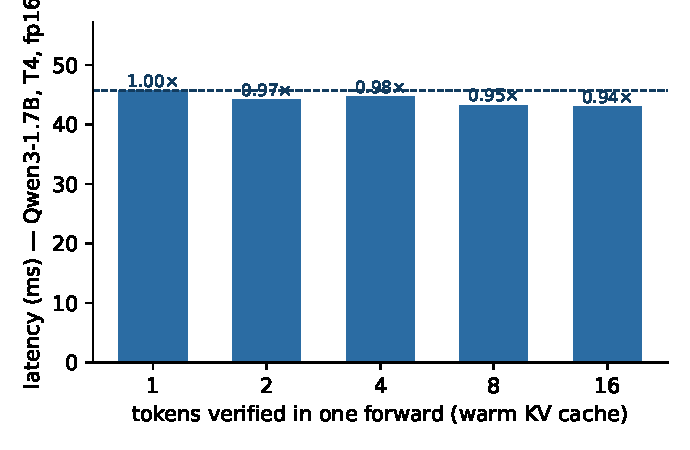
\includegraphics[width=0.5\linewidth]{figs/p5fig2_micro.pdf}
\caption{The conversion factor, measured: best-of-30 latency of one forward over $k$ tokens with a warm KV cache (Qwen3-1.7B, T4, fp16). Sixteen tokens verify in $0.94\times$ the time of one.}
\label{fig:micro}
\end{figure}

Figure~\ref{fig:micro}: $c(16)/c(1) = 0.94$ on the T4 ($45.7 \to 43.1$\,ms). Single-batch decoding at these model sizes is latency-bound; a verified block is as cheap as a single step, so acceptance converts to wall-clock speed at face value. The same measurement explains the CPU ceiling: there, $c(k)$ grows nearly linearly, and our best CPU speedup ($\times$1.41 on the 0.6B) came almost entirely from per-call overhead.

\subsection{End-to-end: the state accelerates every target that carries it}\label{sec:speed}

\begin{figure}[t]
\centering
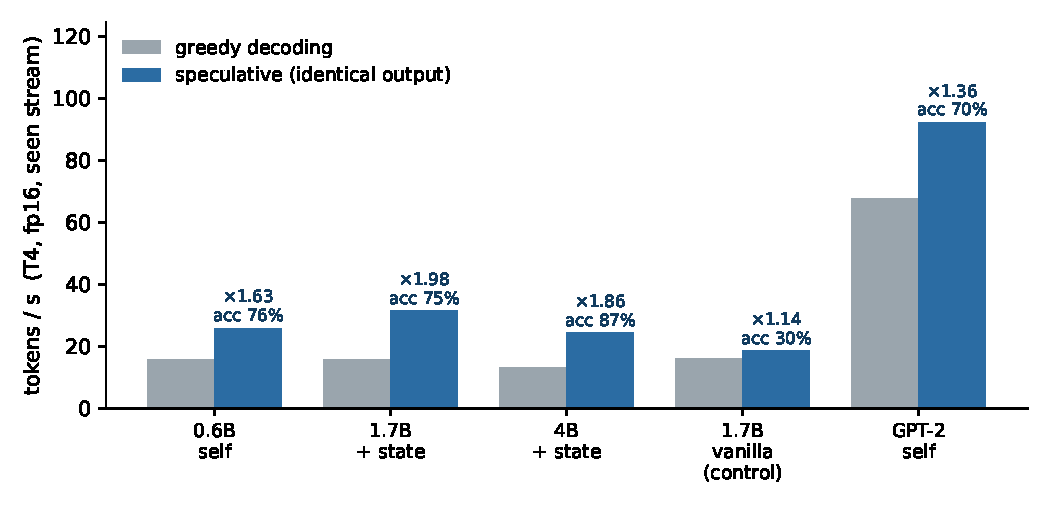
\includegraphics[width=0.95\linewidth]{figs/p5fig1_speedups.pdf}
\caption{End-to-end throughput on seen streams (T4, fp16), plain greedy vs speculative with the state as drafter. Outputs are identical within each pair. The vanilla control (fourth group) shows the boundary: without the memory in the target, there is little to accelerate.}
\label{fig:speed}
\end{figure}

\begin{table}[t]
\centering\small
\caption{Wall-clock summary (T4, fp16; unseen = the 5-prompt control). Speedup is speculative over plain within the same configuration; outputs identical (see \S\ref{sec:negative} for the GPT-2 fp16 caveat).}
\label{tab:speed}
\begin{tabular}{@{}lccccc@{}}
\toprule
configuration & plain $\to$ spec (tok/s) & speedup & acceptance & fwd/token & unseen\\
\midrule
0.6B self & $15.9 \to 25.9$ & $\times$\textbf{1.63} & 76\% & 0.65 & $\times$1.03\\
1.7B $+$ state (calibrated) & $15.9 \to 31.5$ & $\times$\textbf{1.98} & 75\% & 0.52 & $\times$1.09\\
4B $+$ state (auto-calibrated) & $13.1 \to 24.4$ & $\times$\textbf{1.86} & 87\% & 0.55 & $\times$1.00\\
1.7B vanilla (control) & $16.2 \to 18.5$ & $\times$1.14 & 30\% & 0.95 & $\times$0.97\\
GPT-2 self & $67.7 \to 92.3$ & $\times$1.36 & 70\% & 0.77 & $\times$1.01\\
\bottomrule
\end{tabular}
\end{table}

Table~\ref{tab:speed} and Figure~\ref{fig:speed} are the headline. On document-grounded generation, the three augmented Qwen3 targets gain $\times$1.63--1.98 with outputs bit-identical to plain decoding --- the calibrated 1.7B reaches $\times$1.98 at $0.52$ target forwards per emitted token, and the 4B converts its 87\% acceptance despite being the largest and slowest target. The controls hold in both directions: the vanilla 1.7B gains only $\times$1.14 (its distribution does not follow the documents, so drafts miss), and on unseen text no configuration pays more than noise ($\times$0.97--1.09) --- the drafter abstains where the state knows nothing, so \emph{speculation never costs}.

One loop optimization was worth measuring explicitly. Our first loop spent two forwards per drafted round (block verification, then one for the emitted token); fusing them --- each round's verification chunk is $[\text{emitted}] + \text{drafts}$, the standard speculative shape --- costs nothing in output (identity re-verified) and raised $\times$1.54/1.69/1.66 to the $\times$1.63/1.98/1.86 above. The gain matches its own prediction: round statistics from the two-pass runs bound the fused speedups at $\times$1.70/2.02/1.90, and the measurements land within 2--4\% of those bounds at the Qwen3 sizes --- there is little left in the loop. Both generations of runs are archived (\texttt{drafter\_gpu\_*.json} fused, \texttt{*\_twopass.json} prior).

\subsection{The readout must live on the accelerator}\label{sec:ondevice}

Our first GPU runs used the reference numpy readout and were \emph{slower} speculative than plain ($\times$0.62--0.88) --- despite 75--87\% acceptance and the free verification of \S\ref{sec:micro}. The account: plain 0.6B decoding ran at 5.6\,tok/s $=$ 178\,ms/token, of which the GPU forward is only 44\,ms; the remaining $\sim$130\,ms were the vocabulary-sized readout ($V u$ scoring, softmaxes and mixing over 151{,}936 entries, several times per position) on the host's two cores --- negligible on a 16-thread workstation, dominant there, and \emph{paid per drafted position} by speculation. Porting the hot path to the device (keys as int8 hypervectors, values fp16, batched verification of the whole block in one call; the cold store stays a host-side dictionary) removed the bottleneck: plain throughput itself tripled ($5.6 \to 17.6$\,tok/s on the 0.6B in that session; T4 throughput varies by a few tok/s between sessions, visible across our runs), and every speedup of Table~\ref{tab:speed} followed with acceptance figures unchanged to the token. The general statement: with modern vocabularies, any memory that scores tokens must be resident where the model is --- a readout cheap enough to ignore at profiling scale on one machine can silently invert a paper's conclusion on another.

\section{Negative results}\label{sec:negative}

\textbf{(1) A looser draft gate hurts both metrics.} Dropping the matrix gate from the $q_{75}$ to the $q_{60}$ confidence quantile raised draft volume ($163 \to 282$ on GPT-2/CPU) but collapsed acceptance ($75\% \to 48\%$) and speed ($\times$1.17 $\to$ $\times$1.03). Wrong drafts are not free --- they occupy verified positions --- and the readout's own abstention threshold, tuned for prediction, turns out to be the right drafting gate as well. Precision beats coverage.

\textbf{(2) A vanilla target cannot be usefully accelerated.} Configuration B is the clean refutation: with the memory absent from the target's distribution, the 1.7B regenerates $0.4$ words of the source, accepts 30\% of drafts, and gains $\times$1.10. A drafter can only accelerate beliefs its target already holds; the state must be \emph{in} the target for its drafts to land. Acceleration and recall are one purchase, not two.

\textbf{(3) fp16 argmax ties break exact identity on GPT-2.} In fp16, block verification and token-by-token decoding accumulate differently; on GPT-2, whose half-precision logits produce near-ties, 2 of 15 prompts diverged from the plain output (9/10 seen, 4/5 unseen identical). All 60 Qwen3 generations were identical. The guarantee should be stated as ``identical up to fp16 argmax ties'' --- or verification run in fp32 --- on architectures not trained in half precision.

\textbf{(4) Greedy degeneration flatters prompt-lookup.} In our earliest CPU runs, prompt-lookup reached $\times$1.33--1.58 on GPT-2 --- above the persistent drafter. Inspection showed why: greedy GPT-2 degenerates into loops (``\texttt{| | | |}''; ``a.k.a.\ a,k.a.''), which prompt-lookup then copies with near-perfect acceptance. Its advantage partly measures the pathology of the decoding, not knowledge of the text. Any evaluation of retrieval drafters on open-ended greedy generation should report degeneration or use models and lengths where it is controlled; on Qwen3, which degenerates far less, the ordering reverses (76\% vs 50\% acceptance).

\section{Discussion}

\textbf{One state, three currencies.} The companion papers bought prediction with this state; this paper buys recall-for-the-family and wall-clock speed with the same bytes, unchanged. The three purchases share one signal: the surprise-gated writes that make the state predictive are what make its drafts acceptable, and the confidence machinery that decides when the memory may speak is what decides when it may draft. Nothing was added but a verification loop.

\textbf{Read with the small model, serve the family.} Reading is the expensive operation (one forward per token); recall and speed are cheap. The economics this suggests: let the smallest family member read continuously and write the state; let any larger sibling load it, spend two minutes of read-only calibration, and both remember the documents and generate faster on them. Against Cartridges \cite{cartridges}, which trains a per-corpus artifact offline on an accelerator, this is the gradient-free, single-pass, CPU-writable point of the design space; against SuffixDecoding \cite{suffix}, whose trees grow server-side per deployment, it is the bounded, portable, reading-derived one.

\textbf{What the boundary looks like.} Configuration B is the honest edge: the mechanism sells recall-plus-speed on content the state has read, to targets that carry the state. It does not accelerate arbitrary generation (unseen controls: $\times$0.99--1.13), and it does not improve targets that refuse the memory. The regime is the same one the companion papers mapped --- structured, repetitive, or re-visited text --- now priced in tokens per second.

\section{Limitations}

One state per experiment family (two manuscripts; four preprints) and 10 seen prompts per configuration --- widths, not depths; no multi-seed replication of the drafting runs (the underlying memory effects are 5-seed replicated in \cite{sillage,router}); greedy decoding only (speculative \emph{sampling} \cite{leviathan,chen} preserves distributions, not tokens, and is untested here); the 24-word-prompt, 28-token-generation workload is document-grounded completion, favorable to the mechanism and stated as such; cross-model transfer requires a shared tokenizer (the Qwen3 family here) and transfers neither the adapter nor, presumably, states across tokenizers; and the T4 numbers are single-GPU, batch-1 --- server batching changes the latency accounting entirely.

\section{Conclusion}

A fixed-size Hebbian state written by a 0.6B model while reading two documents makes a 4B model that never read them recall them (calibrated read-only in two minutes, settings stable across the family) and makes three model sizes generate $\times$1.6--2.0 faster on that content with outputs identical to normal decoding --- while controls show the memory silent and costless where it knows nothing, and a vanilla target shows the two purchases are one. The oldest speculative idea --- guess cheap, verify exact --- composes with the oldest memory --- write what surprised you --- into a loop where the same 25\,MB pays for prediction, for the family's recall, and for its own inference bill.

\appendix

\section{Reproduction}

\begingroup\emergencystretch=3.5em
Scripts: \texttt{spec/sillage\_drafter.py} (drafters, exact block verification, numpy reference engine), \texttt{spec/torch\_readout.py} (device-resident engine; cross-checked against the reference token-for-token including cold-store rounds), \texttt{spec/bench\_gpu.py} (configurations \texttt{micro}/\texttt{A}/\texttt{B}/\texttt{C}/\texttt{gpt2}, with \texttt{--calibrate} implementing \S\ref{sec:transfermethod}), plus the Kaggle kit used for the T4 runs, assembled from the repository and two documents of your own by \texttt{spec/kaggle/make\_kit.py}. Committed results: fourteen JSON files under \texttt{results/} with the \texttt{drafter\_} prefix --- the T4 microbenchmark, one \texttt{gpu\_*} file per configuration (fused loop; the pre-fusion runs kept as \texttt{*\_twopass}), the read-only calibration (\texttt{calib\_17b}), and the two CPU campaigns (\texttt{cpu\_cross}, \texttt{cpu\_gpt2}). Settings: $\gamma = 8$; cold gate $p \ge 0.35$, min count 2; matrix gate $=$ $q_{75}$ of the state's rolling confidence reservoir, $\le 2$ consecutive; readout grids and abstention exactly as in \cite{sillage}; calibration window $=$ first 20\% of lifetime tokens, stride 3; prompts: 24 words, fixed seeds, 28 generated tokens, greedy; fp16 on GPU, fp32 on CPU. Figures regenerate via \texttt{figures/make\_figures\_p5.py}.\par\endgroup

\begin{thebibliography}{18}\small

\bibitem{sillage} A.~Sghairi. Sillage: Surprise-gated amplitude memory for frozen language models. Preprint, 2026. \href{https://doi.org/10.5281/zenodo.22079016}{doi:10.5281/zenodo.22079016}.

\bibitem{router} A.~Sghairi. Route the scores, not the keys: Gradient-free semantic memory for frozen language models. Preprint, 2026. \href{https://doi.org/10.5281/zenodo.22079444}{doi:10.5281/zenodo.22079444}.

\bibitem{hier} A.~Sghairi. One signal, three tiers: A routed memory hierarchy with surprise-gated consolidation. Preprint, 2026. \href{https://doi.org/10.5281/zenodo.22079471}{doi:10.5281/zenodo.22079471}.

\bibitem{fw} A.~Sghairi. Memory remembers, fast weights adapt: Two gradient-free ways to learn at test time, and why they add up. Preprint, 2026. \href{https://doi.org/10.5281/zenodo.22079481}{doi:10.5281/zenodo.22079481}.

\bibitem{leviathan} Y.~Leviathan, M.~Kalman, Y.~Matias. Fast inference from transformers via speculative decoding. \emph{ICML}, 2023.

\bibitem{chen} C.~Chen, S.~Borgeaud, G.~Irving, J.-B.~Lespiau, L.~Sifre, J.~Jumper. Accelerating large language model decoding with speculative sampling. arXiv:2302.01318, 2023.

\bibitem{pld} A.~Saxena. Prompt lookup decoding. \href{https://github.com/apoorvumang/prompt-lookup-decoding}{github.com/apoorvumang/prompt-lookup-decoding}, 2023.

\bibitem{rest} Z.~He, Z.~Zhong, T.~Cai, J.~D.~Lee, D.~He. REST: Retrieval-based speculative decoding. \emph{NAACL}, 2024.

\bibitem{suffix} G.~Oliaro, Z.~Jia, D.~Campos, A.~Qiao. SuffixDecoding: Extreme speculative decoding for emerging AI applications. \emph{NeurIPS}, 2025 (arXiv:2411.04975).

\bibitem{nest} M.~Li, X.~Chen, A.~Holtzman, B.~Chen, J.~Lin, W.-t.~Yih, X.~V.~Lin. Nearest neighbor speculative decoding for LLM generation and attribution. \emph{NeurIPS}, 2024.

\bibitem{omnidraft} R.~Kinattinkara~Ramakrishnan, Z.~Yuan, S.~Zhuo, C.~Feng, Y.~Lin, C.~Su, X.~Zhang. OmniDraft: A cross-vocabulary, online adaptive drafter for on-device speculative decoding. \emph{NeurIPS}, 2025 (arXiv:2507.02659).

\bibitem{khandelwal2020} U.~Khandelwal, O.~Levy, D.~Jurafsky, L.~Zettlemoyer, M.~Lewis. Generalization through memorization: Nearest neighbor language models. \emph{ICLR}, 2020.

\bibitem{titans} A.~Behrouz, P.~Zhong, V.~Mirrokni. Titans: Learning to memorize at test time. arXiv:2501.00663, 2025.

\bibitem{ttt} Y.~Sun et al. Learning to (learn at test time): RNNs with expressive hidden states. arXiv:2407.04620, 2024.

\bibitem{cartridges} S.~Eyuboglu, R.~Ehrlich, S.~Arora, N.~Guha, D.~Zinsley, E.~Liu, W.~Tennien, A.~Rudra, J.~Zou, A.~Mirhoseini, C.~R\'e. Cartridges: Lightweight and general-purpose long context representations via self-study. arXiv:2506.06266, 2025.

\bibitem{gpt2} A.~Radford, J.~Wu, R.~Child, D.~Luan, D.~Amodei, I.~Sutskever. Language models are unsupervised multitask learners. OpenAI Technical Report, 2019.

\bibitem{qwen3} A.~Yang et al. Qwen3 technical report. arXiv:2505.09388, 2025.

\end{thebibliography}

\end{document}
